\documentclass[11pt,xcolor=dvipsnames]{beamer}
\usetheme{nelle}
\usepackage{natbib}                 % Fancy bibliography.
\usepackage{url}                    % Allow printing of URLs.
\usepackage{outlines}
\usepackage{enumitem}
\usepackage{multicol}
\usepackage{dsfont}
\usepackage{amsmath}
\usepackage{epstopdf}
\usepackage{color}
\usepackage[utf8]{inputenc}

\setbeamerfont{caption}{size=\scriptsize}
\setbeamertemplate{navigation symbols}{}
\setbeamertemplate{footline}[frame number]{}

\def\newblock{\hskip .11em plus .33em minus .07em}

\title{\textbf{Apprentissage statistique en haute dimension}\\
{\large Structures, régulations, et fonction des génomes.}}
\subtitle{Candidature CR-CN en Section 07 au LIRIS (Team Beagle)}
\author[Varoquaux Nelle]{%
Nelle Varoquaux}
\date{28 Mars, 2019}
\institute{Department of Statistics, University of California, Berkeley}

\begin{document}
\begin{frame}[t, noframenumbering]
  \maketitle
\end{frame}

\setcounter{framenumber}{0}

\begin{frame}
\frametitle{L'univers de données -omiques}
% TODO RÉSUMÉ DES DONNÉES OMIQUES
% pour mieux comprendre la biologie moléculaire
\end{frame}


\begin{frame}
\frametitle{Profile de recherche}

{\bf \small Un parcours interdisciplinaire}
\vskip-1.3ex
\rule{\dimexpr\paperwidth-1.5cm\relax}{0.4pt}
\begin{itemize}
\footnotesize
\item[-] Ingénieur Centrale Nantes (spécialité info), M2 MVA
\item[-] 2012-2015 Thèse à {\bf Mines ParisTech}, équipe CBIO (enc. J.-P. Vert)
\begin{itemize}
    \scriptsize
    \item[-] Analyse de la structure tri-dimensionnelle du génome à partir de
    données Hi-C
    \item[-] Étude de la structure tri-dimensionnelle du {\em P. falciparum}.
\end{itemize}
\item[-] 2016-2019 Postdoctorat à {\bf UC Berkeley} (enc. E. Purdom)
\begin{itemize}
    \scriptsize
    \item[-] Analyse fonctionnelle pour l'étude de
    données d'expression génique temporelles
    \item[-] Resistance à la sécheresse du sorgho.
\end{itemize}
\end{itemize}

\vspace{2em}
{\bf \small Implication dans des grands consortiums}
\vskip-1.3ex
\rule{\dimexpr\paperwidth-1.5cm\relax}{0.4pt}
\begin{columns}
\begin{column}{0.2\linewidth}
\centering
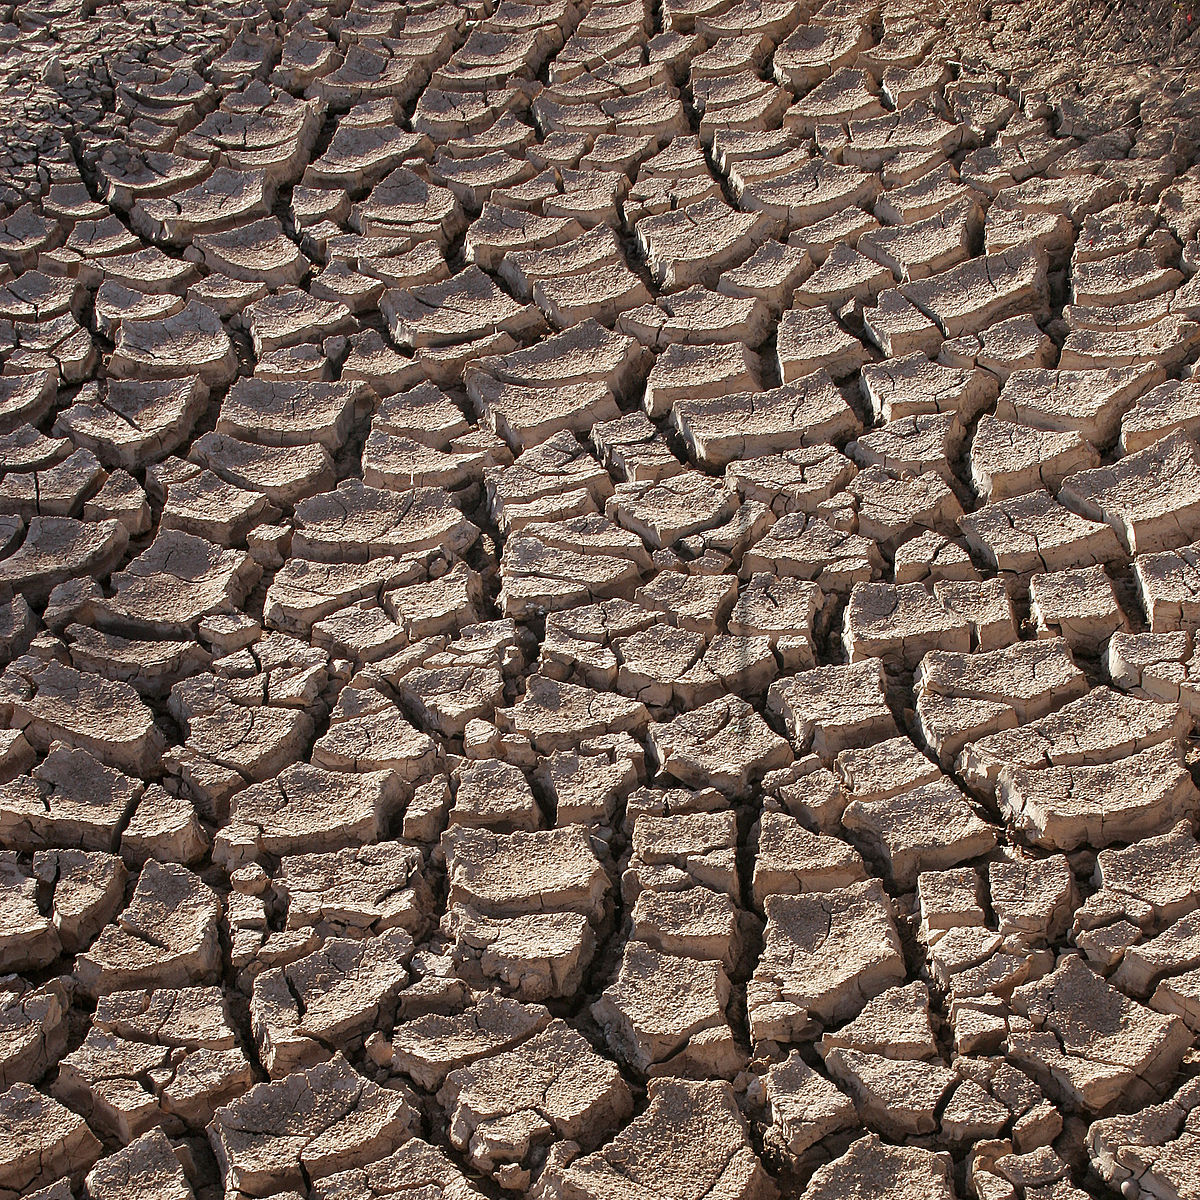
\includegraphics[width=0.9\linewidth]{images/drought_wikipedia_square.png}
\end{column}
\begin{column}{0.8\linewidth}
\begin{itemize}
\footnotesize
\item[-] \textbf{EPICON}\quad EPIgenetic CONtrol of drought resistance in sorghum
\begin{itemize}
\scriptsize
\item[-] 5 instituts de recherche, 8 équipes
\item[-] Étude de la dynamique de la réponse transcriptomique du sorgho sous
stresse de sécheresse.
{\tiny({\color{red}Varoquaux} et al., 2019)}
\end{itemize}
\item[-] \textbf{EMBER}\quad Exploring Maintainer Burnout through Ethnographic
Research
\begin{itemize}
\scriptsize
\item[-] 3 instituts de recherche
\item[-] Dynamique des communautés du logiciel libre ({\tiny Paxton, {\color{red} Varoquaux} et al., 2019, Geiger, {\color{red}
Varoquaux} et al., 2018})
\end{itemize}
\end{itemize}
\end{column}
\end{columns}
\end{frame}

\begin{frame}
\frametitle{Exemple I\quad Inférence de la structure 3D du génome}

\only<1>{
\centering
\includegraphics[width=0.6\linewidth]{figures/yeast_counts.pdf}
}

\end{frame}

\begin{frame}
\frametitle{Example II: Clustering time-course data}
\end{frame}


\begin{frame}
\frametitle{Main contributions}
\end{frame}

\begin{frame}
\frametitle{Research project}
\end{frame}

\begin{frame}
\frametitle{Analysing the 3D structure of DNA}
\end{frame}

\begin{frame}
\frametitle{Causal inference for gene regulatory network inference}
\end{frame}

\begin{frame}
\frametitle{Résumé}
\begin{itemize}
\small
\item[-] {\em Profile de recherche}
\item[-] {\em Programme de recherche} \\
\quad {\centering Apprentissage statistique en haute dimension: structures,
régulations, et fonction des génomes}
\item[-] Adéquation avec les compétences du laboratoire d'accueil
\end{itemize}

\vspace{2em}
{\bf \small Production scentifique}
\vskip-1.3ex
\rule{\dimexpr\paperwidth-1.5cm\relax}{0.4pt}
\begin{itemize}
\small
\item[-] 13 publications de rang A dont 6 premier auteur, 4 deuxième auteur
\item[-] 2 publications soumises, 6 en cours de rédaction
\item[-] Contributions majeurs à 6 logiciels libres (dont
\texttt{scikit-learn}, \texttt{Matplotlib} et \texttt{scikit-image})
\end{itemize}
\end{frame}

\begin{frame}[t, noframenumbering]
\frametitle{Publications}

{\bf \small Publication de rang A, premier auteur}
\vskip-1.3ex
\rule{\dimexpr\paperwidth-1.5cm\relax}{0.4pt}
\begin{itemize}
\small
\item[-] Unfolding the Genome: The Case Study of {\em P. falciparum}. {\color{red}
Varoquaux} (2018)
\item[-] Effective normalization for copy number variation in Hi-C data.
Servant$^*$, {\color{red} Varoquaux$^*$} et al. (2018)
\item[-] Accurate identification of centromere locations in yeast genomes
using Hi-C. {\color{red} Varoquaux} et al. (2015)
\item[-] A statistical approach for inferring the 3D structure of the genome.
{\color{red} Varoquaux} (2014)
\item[-] Three-dimensional modeling of the P. falciparum genome during the
erythrocytic cycle reveals a strong connection between genome architecture and
gene expression. Ay, Bunnik, {\color{red} Varoquaux$^*$} et al. (2014)
\end{itemize}
\end{frame}

\begin{frame}[t, noframenumbering]
\frametitle{Publications}

{\bf \small Publication de rang A, deuxième auteur}
\vskip-1.3ex
\rule{\dimexpr\paperwidth-1.5cm\relax}{0.4pt}
\begin{itemize}
\small
\item[-] The Types, Roles, and Practices of Documentation in Data Analytics
Open Source Software Libraries. Geiger, {\color{red} Varoquaux} et al. (2018)
\item[-] HiC-Pro: an optimized and flexible pipeline for Hi-C data processing.
\quad Servant, {\color{red} Varoquaux} et al. (2015)
\end{itemize}

{\bf \small Autres publications de rang A}
\vskip-1.3ex
\rule{\dimexpr\paperwidth-1.5cm\relax}{0.4pt}
\begin{itemize}
\small
\item[-] Changes in genome organization of parasite-specific gene families
during the Plasmodium transmission stages. \quad Bunnik$^*$, Cook$^*$,
{\color{red} Varoquaux} et al. (2018)
\item[-] Identifying multi-locus chromatin contacts in human cells using
tethered multiple 3C. Ay, Vu, Zeitz, {\color{red} Varoquaux} (2015)
\item[-] A community effort to assess and improve drug sensitivity prediction
algorithms. Costello et al. (2014)
\end{itemize}
\end{frame}

\begin{frame}[t, noframenumbering]
\frametitle{Publications}

{\bf \small Publications soumises}
\vskip-1.3ex
\rule{\dimexpr\paperwidth-1.5cm\relax}{0.4pt}
\begin{itemize}
\item[-] Lifecycle transcriptomics of field-droughted sorghum reveals rapid
biotic and metabolic responses. \quad {\color{red} Varoquaux$^*$}, Cole$^*$,
Gao$^*$ et al. 
\item[-] FIXME pipeline paper 
\end{itemize}

{\bf \small Publications en cours de rédaction}
\vskip-1.3ex
\rule{\dimexpr\paperwidth-1.5cm\relax}{0.4pt}
\begin{itemize}
\item[-] jupyter
\item[-] documentation
\item[-] FOSS with Alex
\item[-] Clustering
\item[-] NB structure
\item[-] Diploid
\end{itemize}


\end{frame}

\begin{frame}[t, noframenumbering]
\frametitle{}
\end{frame}

\end{document}

